\documentclass[11pt,a4paper]{article}

\usepackage[T1]{fontenc}
\usepackage[utf8]{inputenc}
\usepackage{lmodern}
\usepackage[margin=2.5cm]{geometry}
\usepackage{graphicx}
\usepackage{xcolor}
\usepackage{booktabs,tabularx,array}
\usepackage{listings}
\usepackage{tikz}
\usetikzlibrary{arrows.meta,positioning}
\usepackage{float}
\usepackage{caption}
\usepackage{fancyhdr}
\usepackage{titlesec}
\usepackage{enumitem}
\usepackage[hidelinks,colorlinks=true,linkcolor=teal!50!black,urlcolor=teal!50!black]{hyperref}

\definecolor{ink}{HTML}{0B1019}
\definecolor{accent}{HTML}{0E9F8A}
\definecolor{codebg}{HTML}{F4F7FA}
\definecolor{codeframe}{HTML}{C9D3DE}

\titleformat{\section}{\Large\bfseries\color{ink}}{\thesection}{0.8em}{}
\titleformat{\subsection}{\large\bfseries\color{ink}}{\thesubsection}{0.8em}{}
\titlespacing*{\section}{0pt}{2.2ex}{1.2ex}

\pagestyle{fancy}
\fancyhf{}
\fancyhead[L]{\small Sentinel -- Ransomware Metadata Monitoring}
\fancyhead[R]{\small Technical Report}
\fancyfoot[C]{\small\thepage}
\renewcommand{\headrulewidth}{0.3pt}

\lstset{
  basicstyle=\ttfamily\footnotesize,
  backgroundcolor=\color{codebg},
  frame=single, rulecolor=\color{codeframe},
  breaklines=true, columns=fullflexible, keepspaces=true,
  xleftmargin=4pt, xrightmargin=4pt, aboveskip=8pt, belowskip=8pt
}
\captionsetup{font=small,labelfont=bf}
\setlist{itemsep=2pt,topsep=4pt}
\newcommand{\code}[1]{\texttt{\small #1}}

\begin{document}

% ------------------------------------------------------------ title page
\begin{titlepage}
\centering
\vspace*{2.5cm}
{\color{accent}\rule{\linewidth}{1.6pt}}\\[1.2cm]
{\Huge\bfseries Sentinel}\\[0.4cm]
{\Large Ransomware Metadata Monitoring and\\Analyst Investigation Workspace}\\[1.2cm]
{\color{accent}\rule{\linewidth}{0.6pt}}\\[1.6cm]
{\large Technical Report\\[0.3cm] Version 0.4.0}\\[2.2cm]
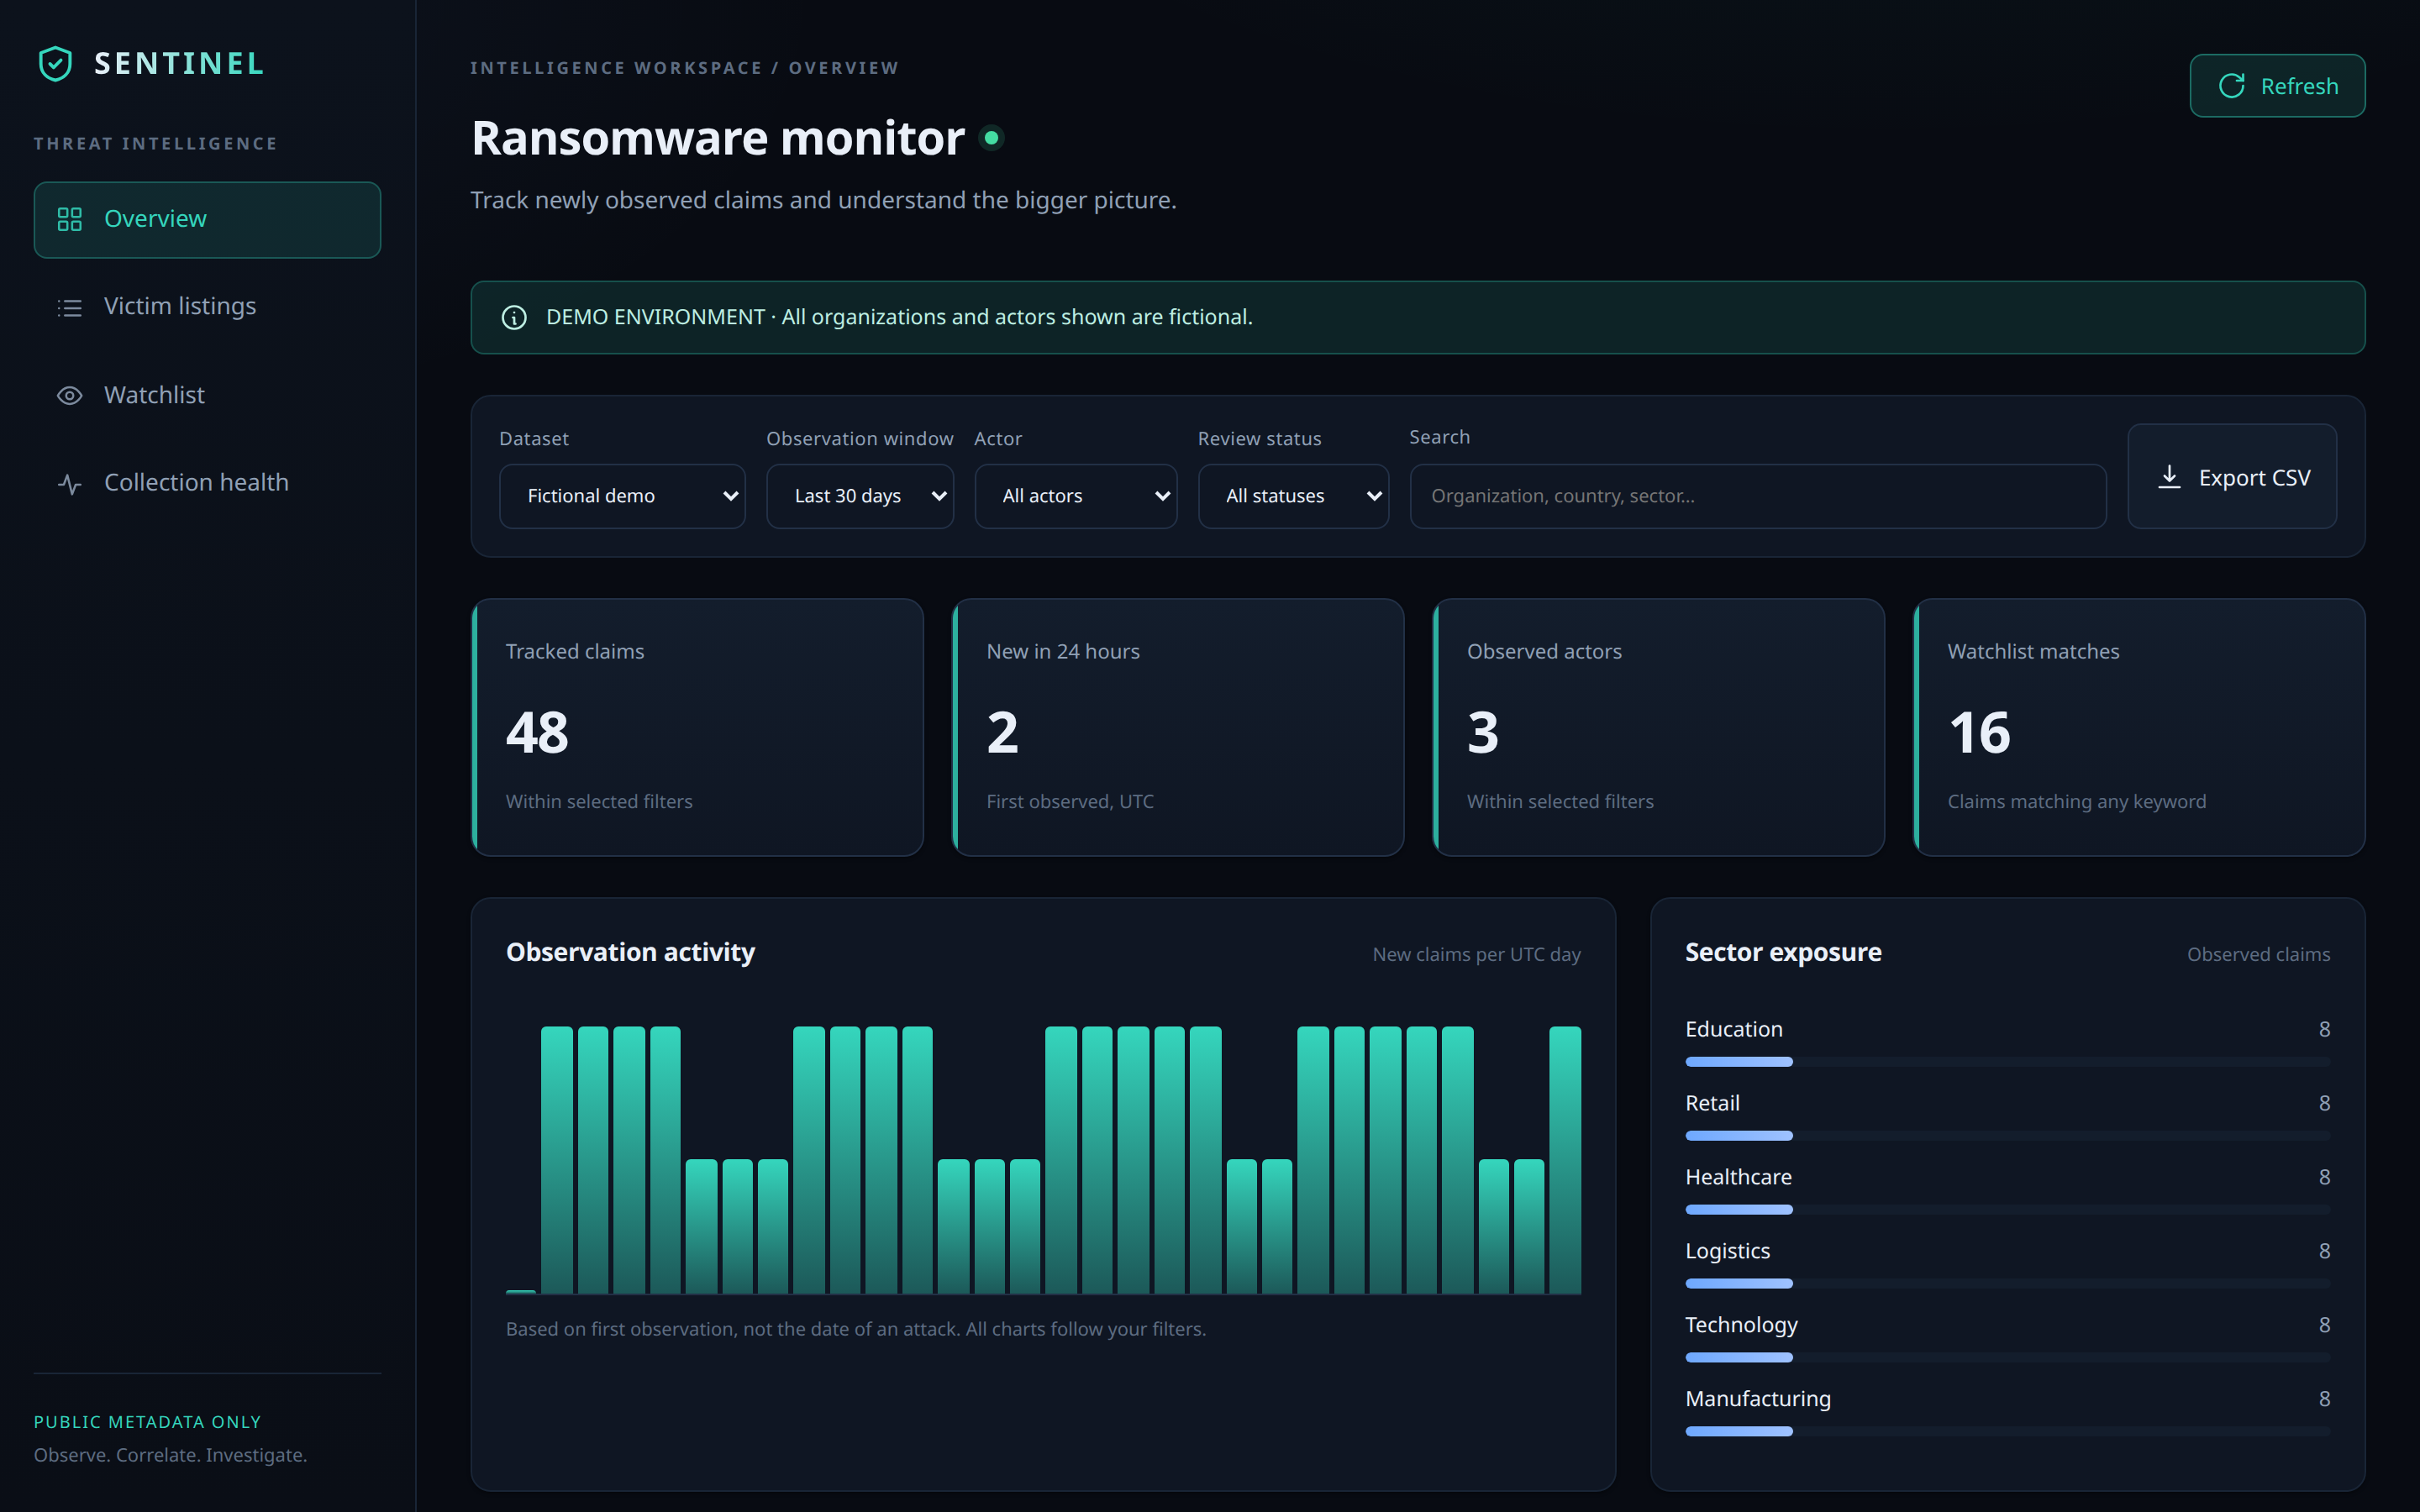
\includegraphics[width=0.92\linewidth]{figures/01_overview.png}\\[1.5cm]
{\large Abdelghany Aitouazghour}\\[0.2cm]
{\normalsize Universit\'e Internationale de Rabat (UIR)}\\[0.6cm]
{\normalsize November 2026}
\vfill
\end{titlepage}

\begin{abstract}
\noindent Sentinel is a local, defensive threat-intelligence tool that collects \emph{public} ransomware leak-site listing metadata, stores it in a normalized SQLite database, and presents it through an analyst dashboard. It records which organizations a threat actor \emph{claims} to have compromised, when each claim was first observed, and from which source. It never downloads stolen data, never executes remote scripts, and never contacts threat actors. This report documents the motivation, architecture, technology stack, data model, collection pipeline, security controls, user interface, testing strategy, and known limitations of version 0.4.0. All figures are produced from a running instance populated with a fictional demonstration dataset.
\end{abstract}

\tableofcontents
\newpage

% ------------------------------------------------------------ 1
\section{Introduction}
Ransomware groups operate public ``leak sites'' where they list organizations they claim to have breached, often as a pressure tactic. These pages change frequently, are spread across many operators, and many are reachable only through Tor. A security analyst who wants to notice newly listed organizations must revisit each page manually and cannot easily answer simple questions such as \emph{when did we first see this claim?} or \emph{did any listing match a sector we protect?}

Sentinel automates the collection and bookkeeping part of this workflow while keeping the judgement part with the analyst. It consolidates listing metadata from multiple sources, gives each claim a stable identity and an auditable first-observation timestamp, and provides a workspace to triage claims with notes and history.

\subsection{Objectives}
\begin{itemize}
  \item Collect listing \emph{metadata only} (organization name, actor, country, sector) from allowlisted public sources.
  \item Deduplicate claims across sources while preserving provenance and first-seen time.
  \item Provide an investigation workflow: status, priority, notes, and an append-only assessment history.
  \item Expose source health honestly, including failures, back-off, and staleness.
  \item Remain safe to operate: bounded network access, no leaked content, loopback-only web interface.
\end{itemize}

\subsection{Scope and ethical boundaries}
A listing is a \emph{claim}, not verified evidence of a breach. The tool therefore labels every record as an unverified claim and never infers that an incident is confirmed. Trends reflect the coverage and publication behaviour of the monitored sources, not total ransomware incidence. The project stores normalized metadata only: no leaked files, no raw page captures, no victim contact details, and no download links.

% ------------------------------------------------------------ 2
\section{Technology Stack}
The project deliberately minimizes dependencies. The dashboard, import, demo generator, database layer, and HTTP server rely solely on the Python standard library. Third-party packages are needed only for network collection and HTML parsing.

\begin{table}[H]
\centering
\renewcommand{\arraystretch}{1.25}
\begin{tabularx}{\linewidth}{@{}l l X@{}}
\toprule
\textbf{Layer} & \textbf{Tool} & \textbf{Purpose} \\
\midrule
Language & Python $\ge$ 3.11 & Collector, store, server, CLI (run locally on 3.14; CI matrix 3.11--3.14) \\
Persistence & SQLite (WAL mode) & Single-file database, transactional writes, 30\,s busy timeout \\
HTTP server & \code{http.server} & \code{ThreadingHTTPServer} bound to loopback, no framework \\
HTTP client & \code{requests[socks]} & Bounded fetch with optional SOCKS5 proxy \\
HTML parsing & \code{beautifulsoup4} & Text-only extraction using CSS selectors \\
CLI & \code{argparse} & Subcommands: \code{demo}, \code{serve}, \code{monitor}, \code{collect}, \code{import}, \code{tor-check} \\
Frontend & HTML, CSS, vanilla JS & No framework, no CDN, no web fonts; inline SVG icon sprite \\
Anonymity & Tor (Docker) & Dedicated local client on Debian bookworm-slim, SOCKS5 on 127.0.0.1:9050 \\
Testing & \code{unittest}, \code{coverage} & 48 tests, 91\% line and branch coverage \\
Packaging & \code{setuptools}, \code{build} & Installable wheel with bundled static assets \\
CI & GitHub Actions & Test matrix, coverage report, JS syntax check, wheel verification \\
Dependency hygiene & Dependabot & Automated update proposals \\
\bottomrule
\end{tabularx}
\caption{Tools and their roles.}
\end{table}

\subsection{Design decision: standard library first}
Avoiding a web framework and ORM keeps the attack surface small, removes transitive dependencies from the request path, and makes every behaviour auditable in a few hundred lines. The trade-off is that features such as authentication, routing, and migrations must be built deliberately; these are documented as out of scope for the local MVP.

% ------------------------------------------------------------ 3
\section{System Architecture}
Sentinel is a linear pipeline from approved sources to a local analyst interface. Collection and presentation share only the SQLite database, so either side can run, fail, or restart independently.

\begin{figure}[H]
\centering
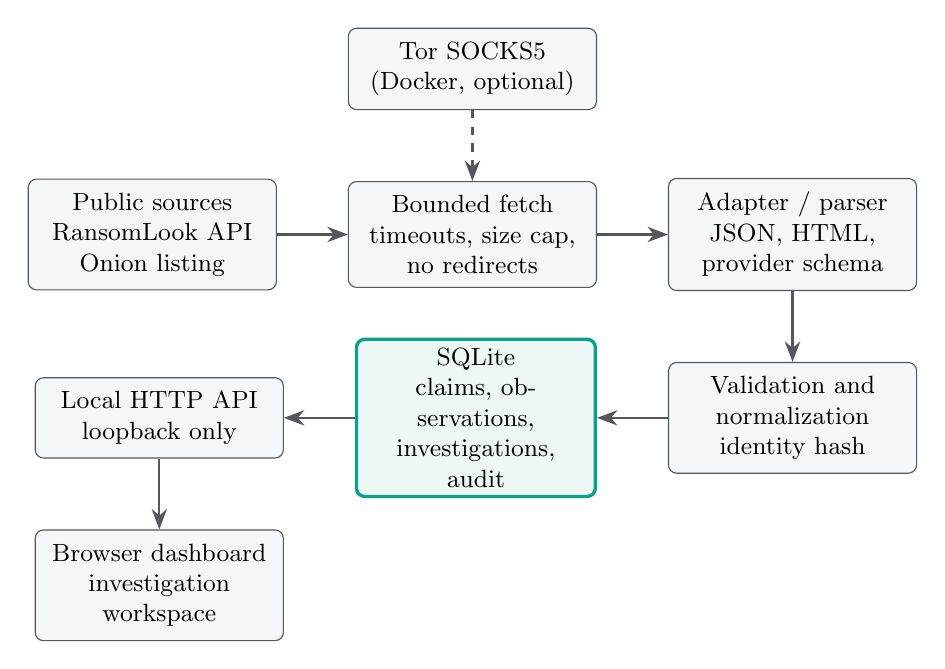
\begin{tikzpicture}[
  font=\small, node distance=0.9cm and 0.9cm,
  box/.style={draw=ink!70, rounded corners=3pt, fill=codebg, minimum height=0.95cm, align=center, inner sep=5pt, text width=2.8cm},
  store/.style={draw=accent, very thick, rounded corners=3pt, fill=accent!8, minimum height=1.1cm, align=center, text width=2.8cm},
  arr/.style={-{Stealth[length=2.6mm]}, thick, ink!70}
]
\node[box] (src) {Public sources\\RansomLook API\\Onion listing};
\node[box, right=of src] (fetch) {Bounded fetch\\timeouts, size cap,\\no redirects};
\node[box, right=of fetch] (parse) {Adapter / parser\\JSON, HTML,\\provider schema};
\node[box, below=of parse] (norm) {Validation and\\normalization\\identity hash};
\node[store, left=of norm] (db) {SQLite\\claims, observations,\\investigations, audit};
\node[box, left=of db] (api) {Local HTTP API\\loopback only};
\node[box, below=of api] (ui) {Browser dashboard\\investigation workspace};
\node[box, above=of fetch] (tor) {Tor SOCKS5\\(Docker, optional)};

\draw[arr] (src) -- (fetch);
\draw[arr] (fetch) -- (parse);
\draw[arr] (parse) -- (norm);
\draw[arr] (norm) -- (db);
\draw[arr] (db) -- (api);
\draw[arr] (api) -- (ui);
\draw[arr, dashed] (tor) -- (fetch);
\end{tikzpicture}
\caption{End-to-end data flow. The dashed edge is used only for onion sources.}
\end{figure}

\subsection{Module responsibilities}
\begin{table}[H]
\centering
\renewcommand{\arraystretch}{1.2}
\begin{tabularx}{\linewidth}{@{}l X@{}}
\toprule
\textbf{Module} & \textbf{Responsibility} \\
\midrule
\code{sentinel/\_\_main\_\_.py} & Command-line entry point, import, demo seeding, scheduler loop, server start-up \\
\code{sentinel/collector.py} & Network controls, JSON and HTML adapters, run logging, exponential back-off \\
\code{sentinel/providers.py} & Allowlisted provider endpoints, authentication header, schema mapping \\
\code{sentinel/tor.py} & Onion v3 address and checksum validation, proxy policy, Tor route diagnostic \\
\code{sentinel/store.py} & Schema and migrations, validation, deduplication, investigations, audit trail \\
\code{sentinel/server.py} & HTTP routes, same-origin enforcement, watchlist mutation, CSV export \\
\code{sentinel/monitor.py} & Runs the dashboard and a periodic collector in one foreground process \\
\code{sentinel/static/} & Dependency-free dashboard: \code{index.html}, \code{app.js}, \code{style.css} \\
\bottomrule
\end{tabularx}
\caption{Source layout (about 1{,}430 lines of Python, JavaScript, HTML and CSS including tests).}
\end{table}

\subsection{Run modes}
\begin{description}
  \item[\code{demo}] Seeds 48 clearly labelled fictional records in an isolated partition.
  \item[\code{serve}] Serves the dashboard and API from the existing database; no network collection.
  \item[\code{collect}] One collection pass, or a repeating foreground worker with an interval of at least 300 seconds.
  \item[\code{monitor}] Dashboard plus a background collector thread that polls configured sources.
  \item[\code{tor-check}] Verifies a local SOCKS route through the Tor Project check service and stores the diagnostic.
\end{description}

% ------------------------------------------------------------ 4
\section{Data Model}
The schema is created idempotently on connection and carries a \code{user\_version} of 4. Additive migrations add columns without disturbing existing rows.

\begin{table}[H]
\centering
\renewcommand{\arraystretch}{1.2}
\begin{tabularx}{\linewidth}{@{}l X@{}}
\toprule
\textbf{Table} & \textbf{Content} \\
\midrule
\code{victims} & One row per tracked claim: identity hash, name, actor, country, sector, first source, claimed publication date, \code{first\_seen}, \code{last\_seen}, demo flag \\
\code{observations} & Per-source provenance for a claim: first and last sighting, sighting count, provider-reported time. Key: (claim, source, URL) \\
\code{investigations} & Analyst status, priority, notes, and an integer \code{version} used for optimistic concurrency \\
\code{audit\_events} & Append-only before/after JSON snapshots of each assessment \\
\code{watchlist} & Unique keywords matched case-insensitively against name, country, sector \\
\code{runs} & Collection attempts with status, counts, and a sanitized error \\
\code{source\_state} & Enabled flag, last attempt and success, next eligible poll, failure count, transport kind \\
\code{transport\_checks} & Latest Tor route diagnostic per proxy \\
\bottomrule
\end{tabularx}
\caption{Database tables.}
\end{table}

\subsection{Claim identity and deduplication}
A claim is identified by a truncated SHA-256 of the demo flag, the case-folded actor, and the case-folded organization name:
\begin{lstlisting}
id = sha256(f"{demo}|{actor.casefold()}|{name.casefold()}")[:24]
\end{lstlisting}
Repeated listings of the same organization by the same actor collapse into one claim. The first source and original metadata are retained; only \code{last\_seen} advances and the per-source sighting counter increments. Name variants and repeat incidents require analyst review, a limitation documented in Section~\ref{sec:limits}.

\subsection{Timestamps}
Three notions of time are kept separate to avoid misleading trends: the \emph{claimed publication date} reported by the source, the \emph{provider observation date} when a feed supplies one, and the local \emph{first-seen} and \emph{last-seen} times generated by the collector. Dashboard activity charts use first observation, not the date of an attack.

% ------------------------------------------------------------ 5
\section{Collection Pipeline}
\begin{enumerate}
  \item Load trusted JSON configuration, validate names, intervals ($\ge 300$\,s) and delays (1--60\,s), and record the active source inventory.
  \item Skip disabled sources and sources whose persisted \code{next\_poll} is still in the future.
  \item Fetch one bounded response (Section~\ref{sec:fetch}).
  \item Parse into normalized records through the matching adapter.
  \item Validate the entire batch; a malformed row fails the whole source atomically.
  \item Insert unseen identities, refresh \code{last\_seen}, upsert the observation.
  \item Log the run, update source state, compute the next poll, then wait the per-source delay.
\end{enumerate}

\subsection{Source adapters}
\begin{description}
  \item[RansomLook] Reads the public recent-post API over HTTPS. A first real synchronization observed 100 records.
  \item[Ransomware.live PRO] Optional; requires an API key supplied through an environment variable. Its authenticated endpoint has not been exercised in this project and the source ships disabled.
  \item[Generic JSON] Expects an array matching the import schema, up to 10{,}000 records.
  \item[Generic HTML] CSS selectors extract text only. A zero-match response is an error so a changed layout is never mistaken for a healthy empty source.
  \item[Onion listing] A direct Tor connection to one public listing page. A live test observed 3 claims, 1 newly inserted.
  \item[Onion status] Availability check only; infers no victim identities.
\end{description}

\subsection{Bounded fetching}\label{sec:fetch}
\begin{itemize}
  \item Only \code{http} and \code{https} URLs without embedded credentials.
  \item Connect timeout 15\,s, read timeout 30\,s, total streaming budget 60\,s.
  \item Decompressed response capped at 2\,MB; content type must match the adapter.
  \item Redirects are never followed; environment proxy settings are ignored.
  \item Providers must match a fixed endpoint allowlist.
\end{itemize}

\subsection{Failure handling}
Errors are recorded as sanitized text that never contains response bodies or credentials. After a failure, the next poll is delayed by exponential back-off, capped at 24 hours, and extended to honour a \code{Retry-After} header. There is no immediate retry loop. Dashboard freshness is derived from the last success: \emph{fresh}, \emph{stale} (older than twice the interval or 30 minutes, whichever is larger), \emph{error}, \emph{never synced}, or \emph{disabled}.

\subsection{Tor transport}
Onion hosts are refused unless a local \code{socks5h://} proxy is configured, which forces hostname resolution through Tor and prevents DNS leaks. Before any request, the v3 onion address is decoded and its checksum verified (SHA3-256 over the public key and version byte). The proxy must be loopback with an explicit port and no credentials. The bundled Docker client runs read-only, drops all Linux capabilities, sets \code{no-new-privileges}, and publishes its port only on 127.0.0.1.

% ------------------------------------------------------------ 6
\section{Web Interface and API}
The server binds exclusively to \code{127.0.0.1}, validates the \code{Host} header against the listening port, and serves a fixed set of static assets.

\begin{table}[H]
\centering
\renewcommand{\arraystretch}{1.2}
\begin{tabularx}{\linewidth}{@{}l l X@{}}
\toprule
\textbf{Method} & \textbf{Route} & \textbf{Result} \\
\midrule
GET & \code{/api/health} & Service status \\
GET & \code{/api/dashboard} & Filtered claims, aggregates, watchlist, sources, recent runs \\
GET & \code{/api/export} & Filtered CSV with formula-prefix neutralization \\
GET & \code{/api/investigation} & One claim with observations and assessment history \\
POST & \code{/api/watchlist} & Add or delete a keyword \\
POST & \code{/api/investigation} & Save an assessment with version check (409 on conflict) \\
\bottomrule
\end{tabularx}
\caption{HTTP API. Query filters: \code{mode}, \code{days} (7/30/90/365), \code{actor}, \code{q}, \code{status}.}
\end{table}

\subsection{Optimistic concurrency}
An assessment save carries the version the browser last read. Inside an immediate transaction the server compares it with the stored version and rejects stale writes with HTTP 409, so two open tabs cannot silently overwrite each other's notes. Every successful save appends a before/after snapshot to the audit table.

% ------------------------------------------------------------ 7
\section{User Interface and Design}
The interface was redesigned for version 0.4.0 around a security-operations aesthetic and a small design system, guided by published UI/UX guidance: SVG icon sets rather than emoji, visible focus states, reduced-motion support, tested breakpoints, and semantic colour tokens. Because the application enforces a strict Content Security Policy, the design is fully self-contained: it uses a system font stack, an inline SVG sprite, and an external stylesheet without inline styles.

\subsection{Design system}
\begin{itemize}
  \item \textbf{Tokens.} Semantic CSS variables for surfaces, text, brand, and status colours; a 4\,px spacing scale; consistent radii and elevation.
  \item \textbf{Hierarchy.} Four summary cards, then activity and sector charts, then the claims table, then watchlist and health.
  \item \textbf{Accessibility.} Skip link, visible focus rings, ARIA live regions for status and errors, \code{prefers-reduced-motion} support, and run status shown by both a colour dot and text.
  \item \textbf{Responsiveness.} Layouts adapt at 1100\,px and 760\,px; the sidebar collapses to a top bar on phones.
  \item \textbf{Honest labelling.} A persistent banner distinguishes fictional demo data from collected metadata and reminds the reader that listings are unverified.
\end{itemize}

\begin{figure}[H]
\centering
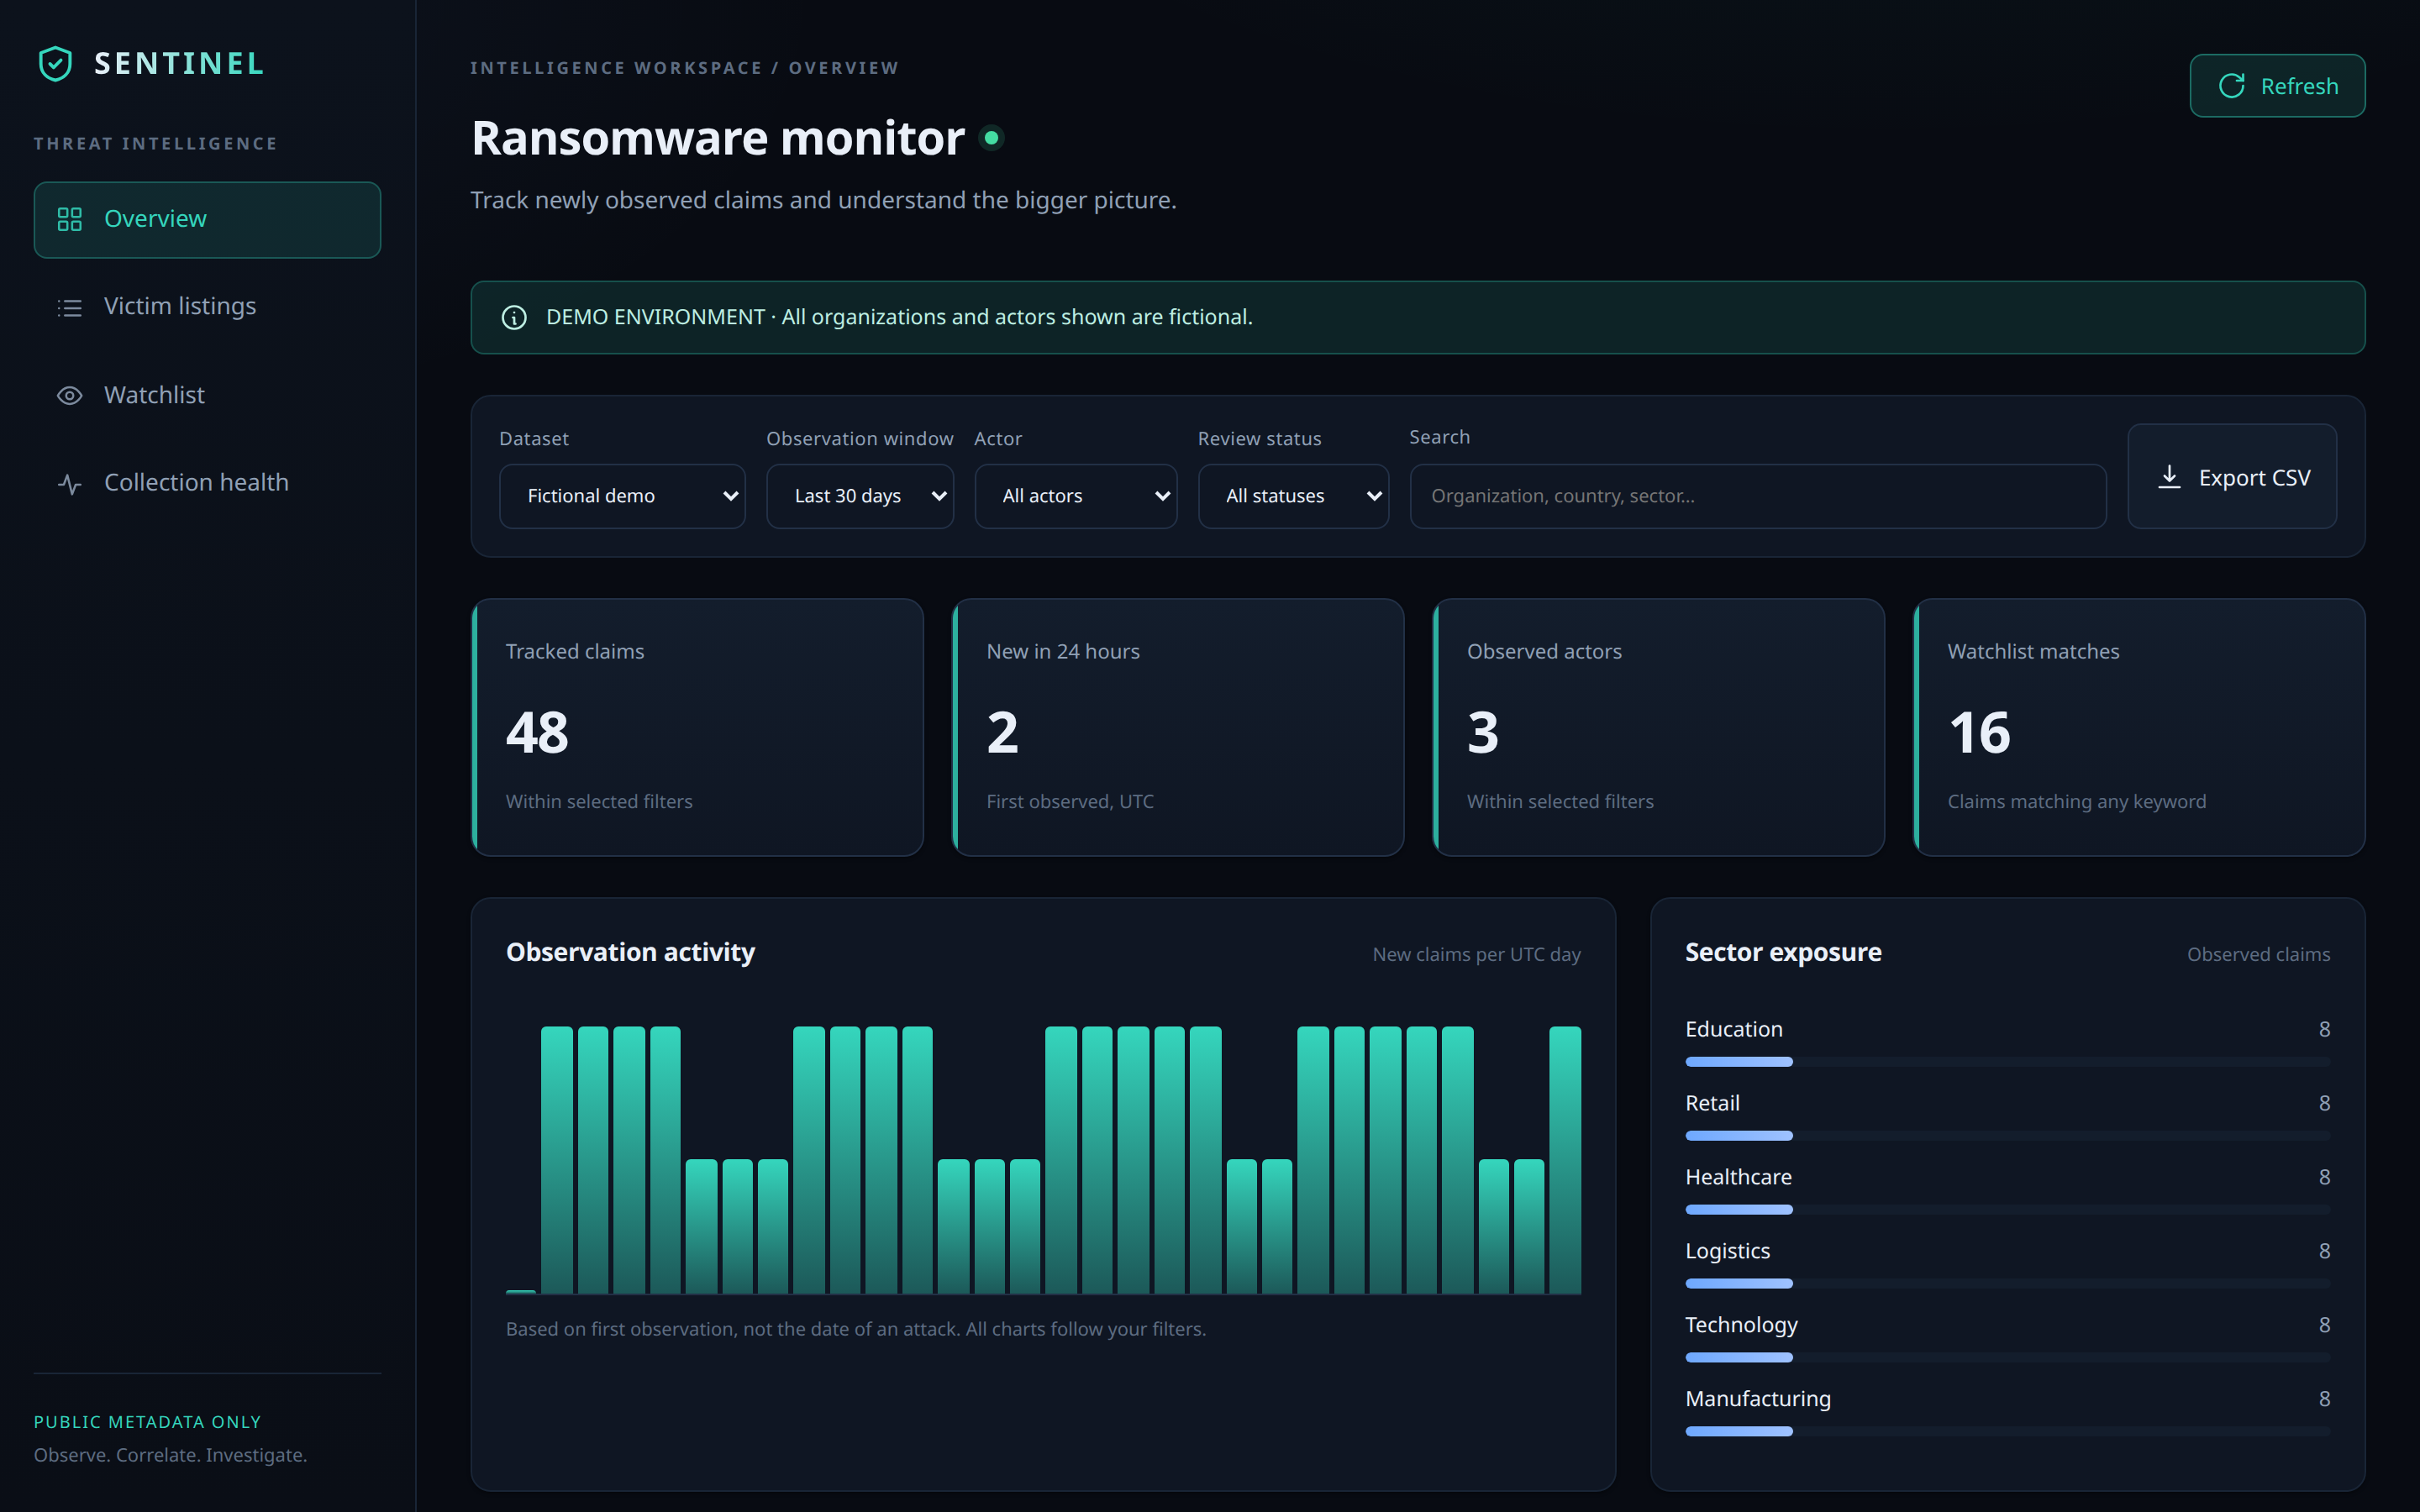
\includegraphics[width=\linewidth]{figures/01_overview.png}
\caption{Overview: filters, summary cards, daily observation activity and sector exposure (fictional demo data).}
\end{figure}

\begin{figure}[H]
\centering
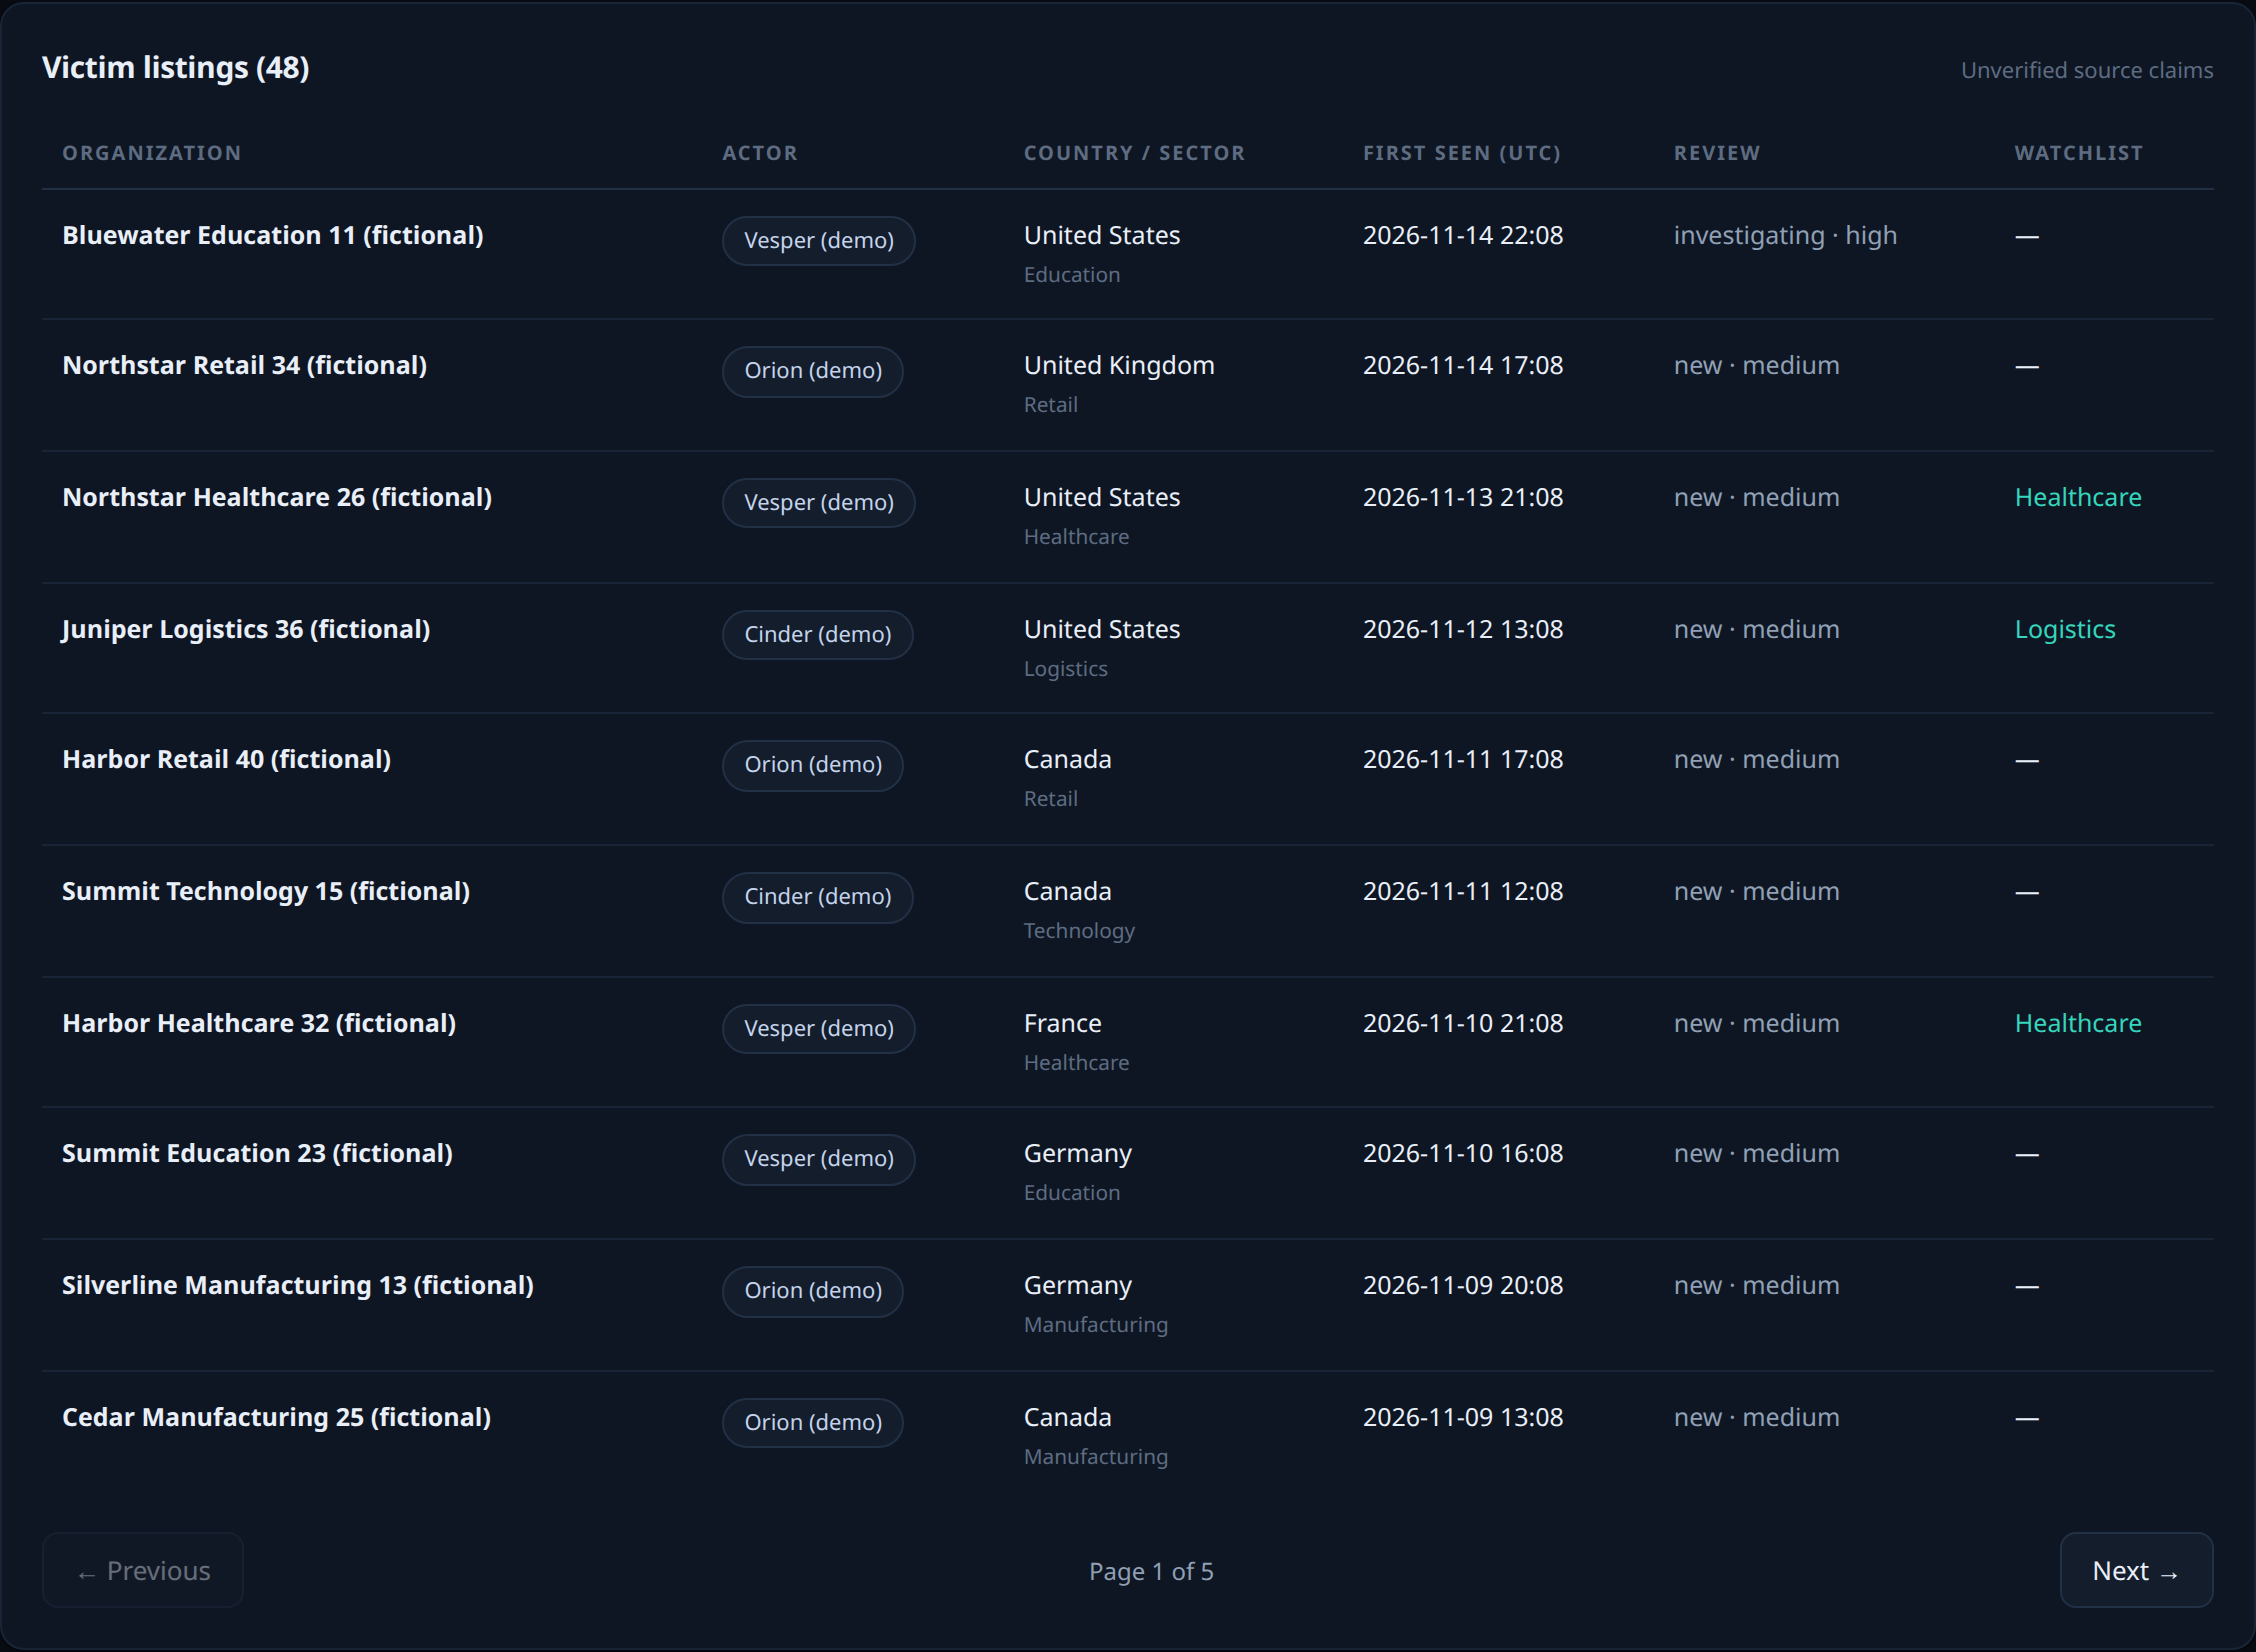
\includegraphics[width=\linewidth]{figures/03_listings.png}
\caption{Victim listings table with actor tags, review status and watchlist matches, paginated ten rows per page.}
\end{figure}

\begin{figure}[H]
\centering
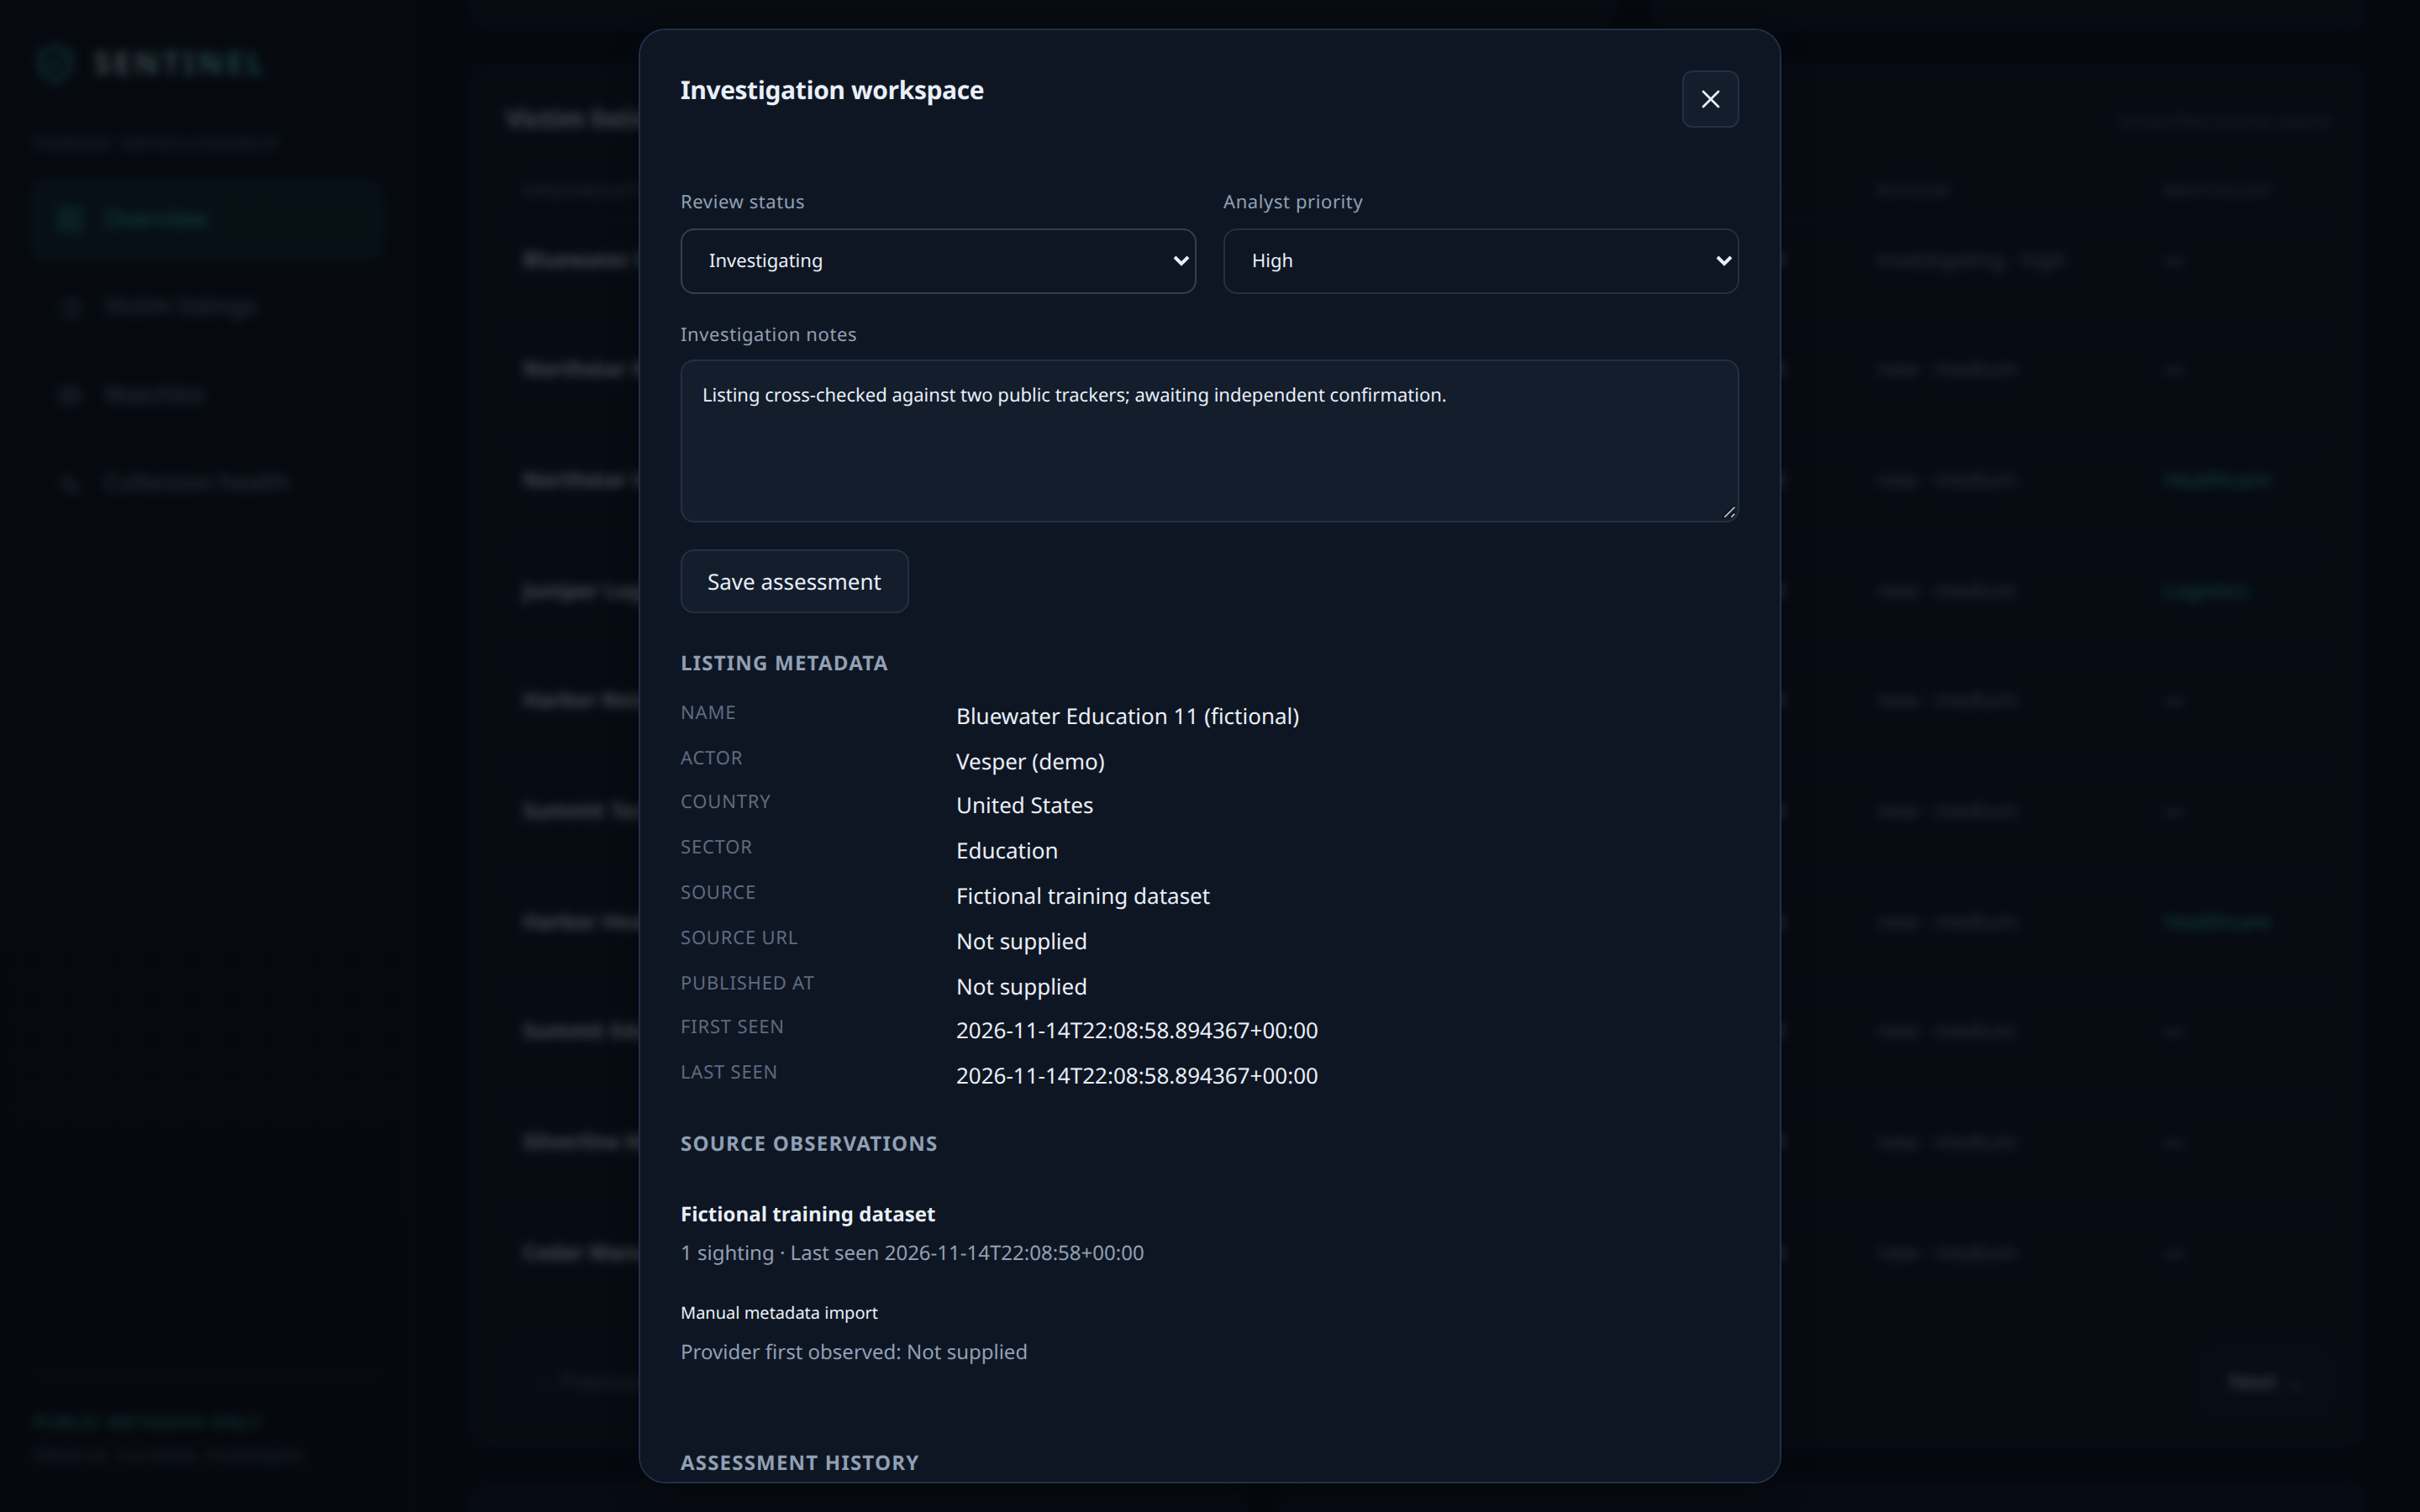
\includegraphics[width=0.82\linewidth]{figures/04_investigation.png}
\caption{Investigation workspace: status, priority, notes, listing metadata, per-source observations, and assessment history.}
\end{figure}

\begin{figure}[H]
\centering
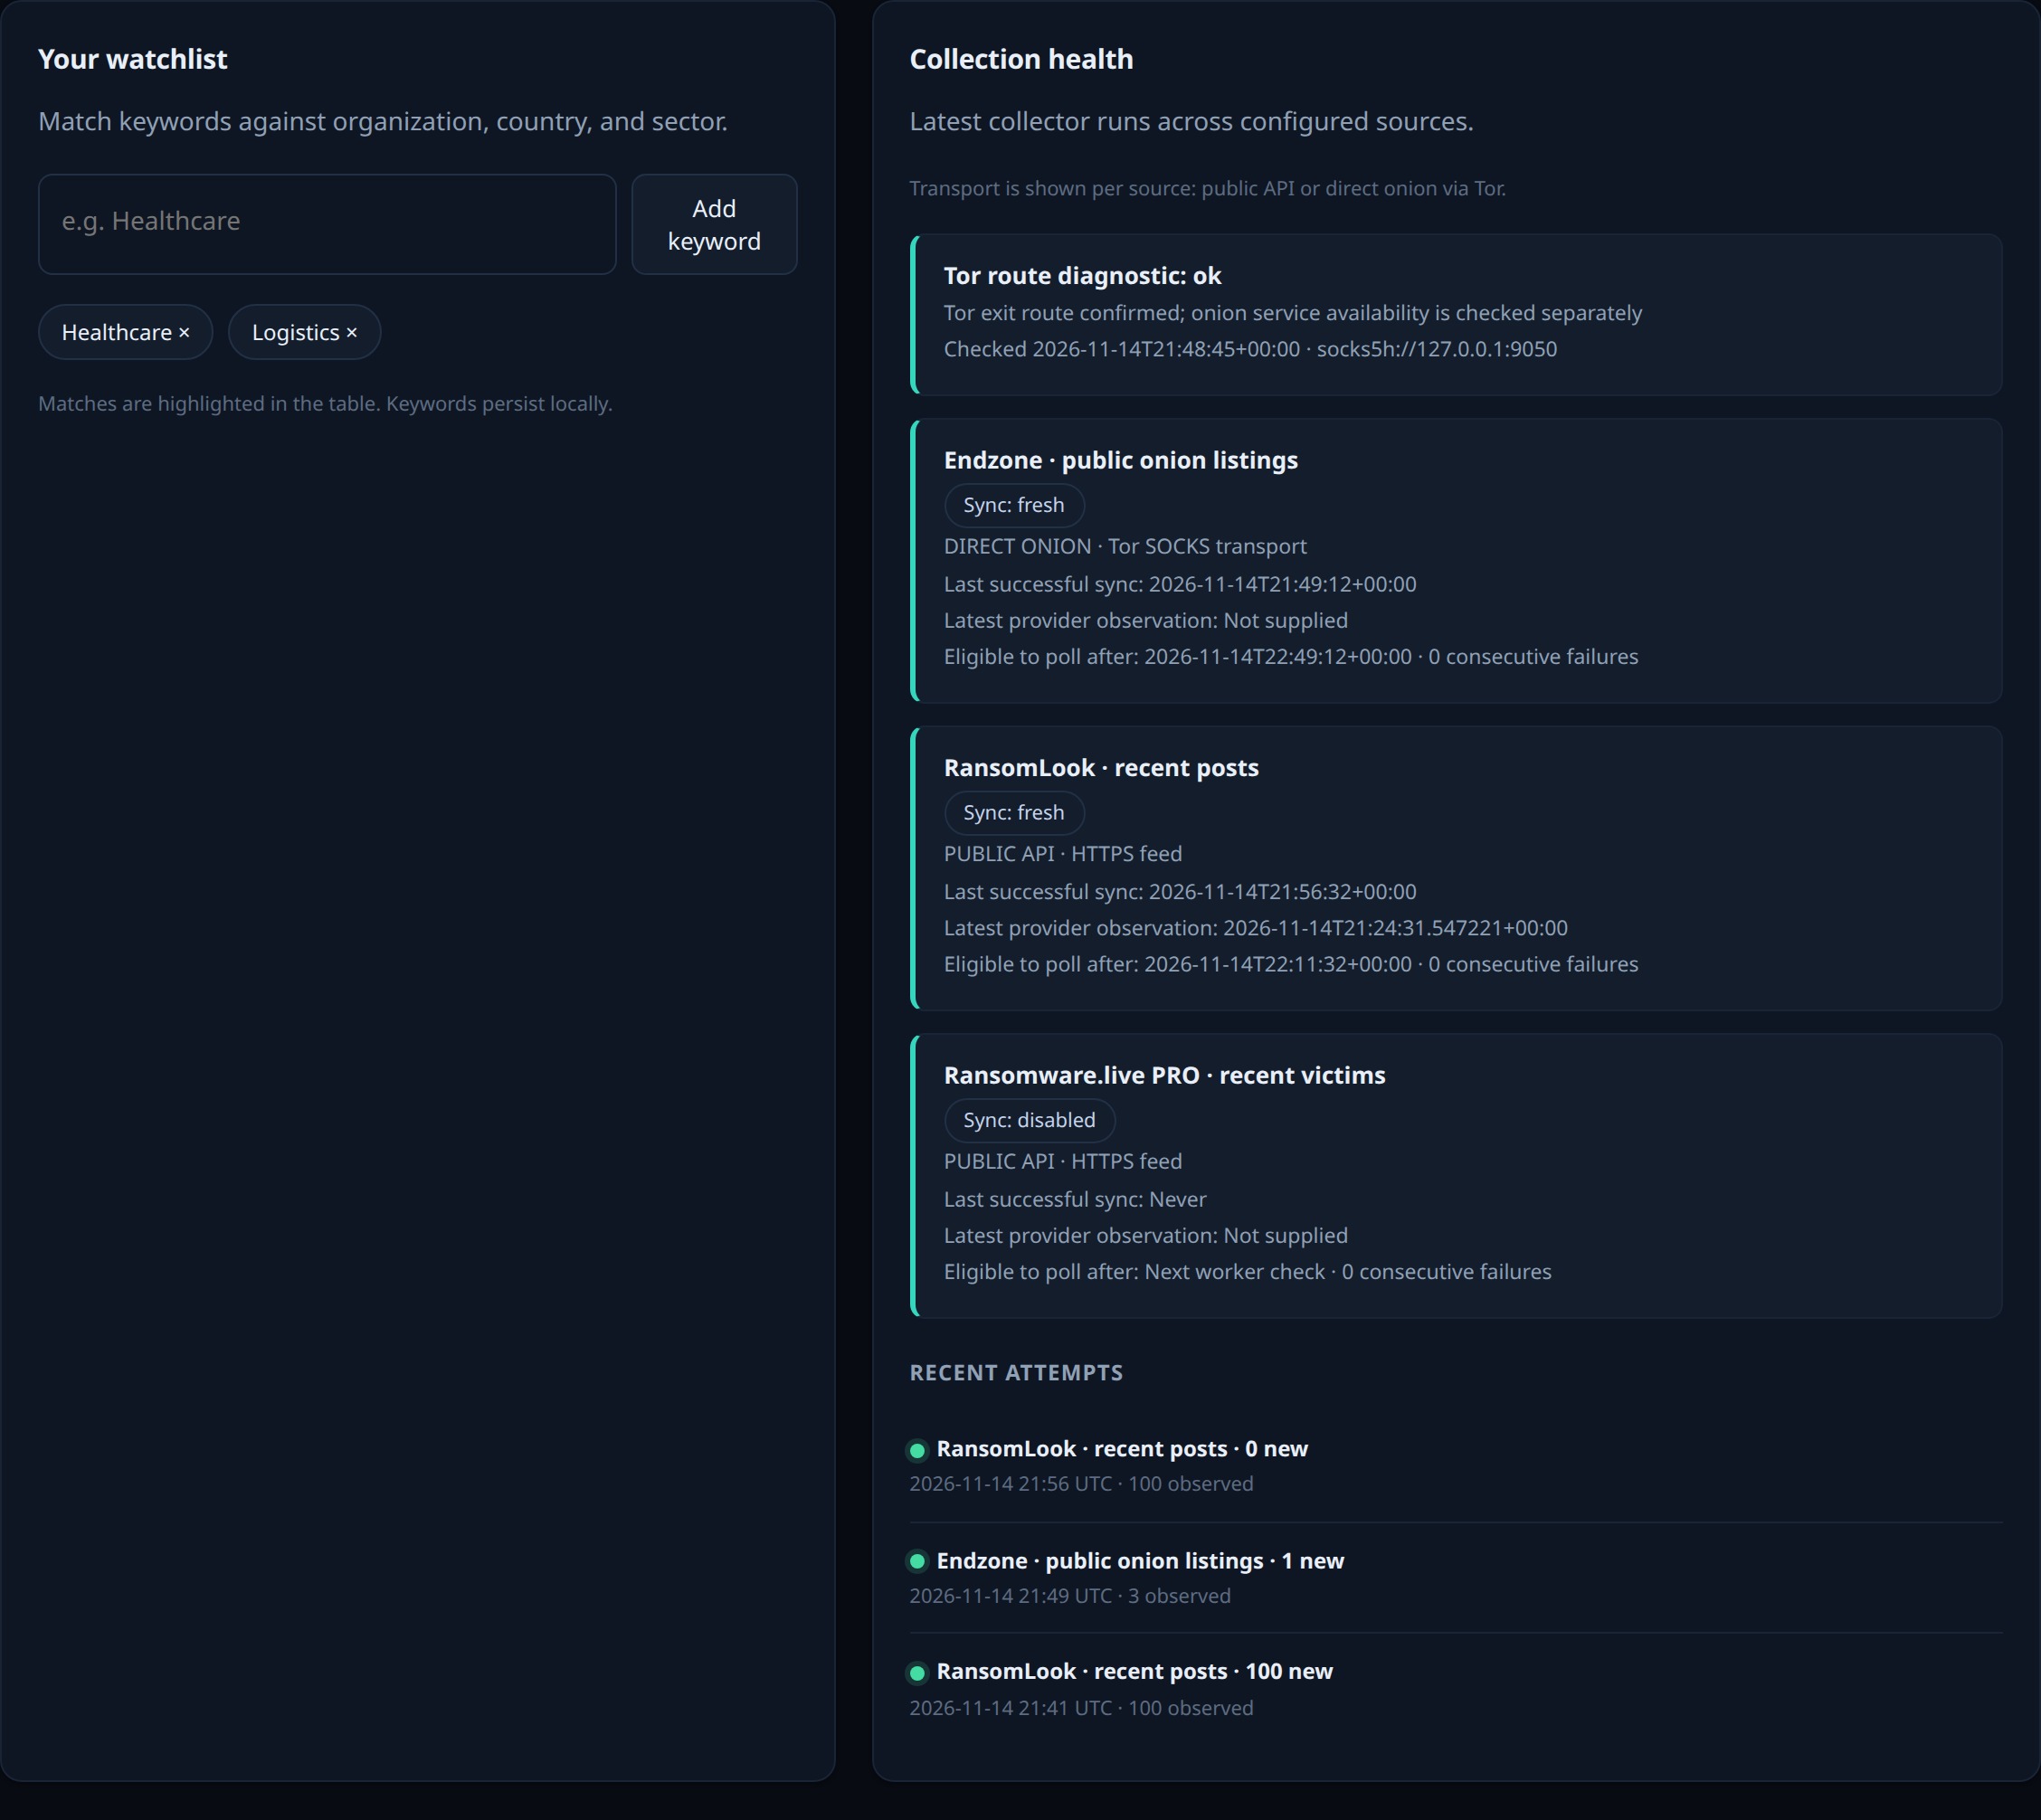
\includegraphics[width=\linewidth]{figures/05_watchlist_health.png}
\caption{Watchlist keywords and collection health. The panel shows the Tor route diagnostic, each source's freshness and transport, and recent runs. The health data comes from an actual collection history.}
\end{figure}

\begin{figure}[H]
\centering
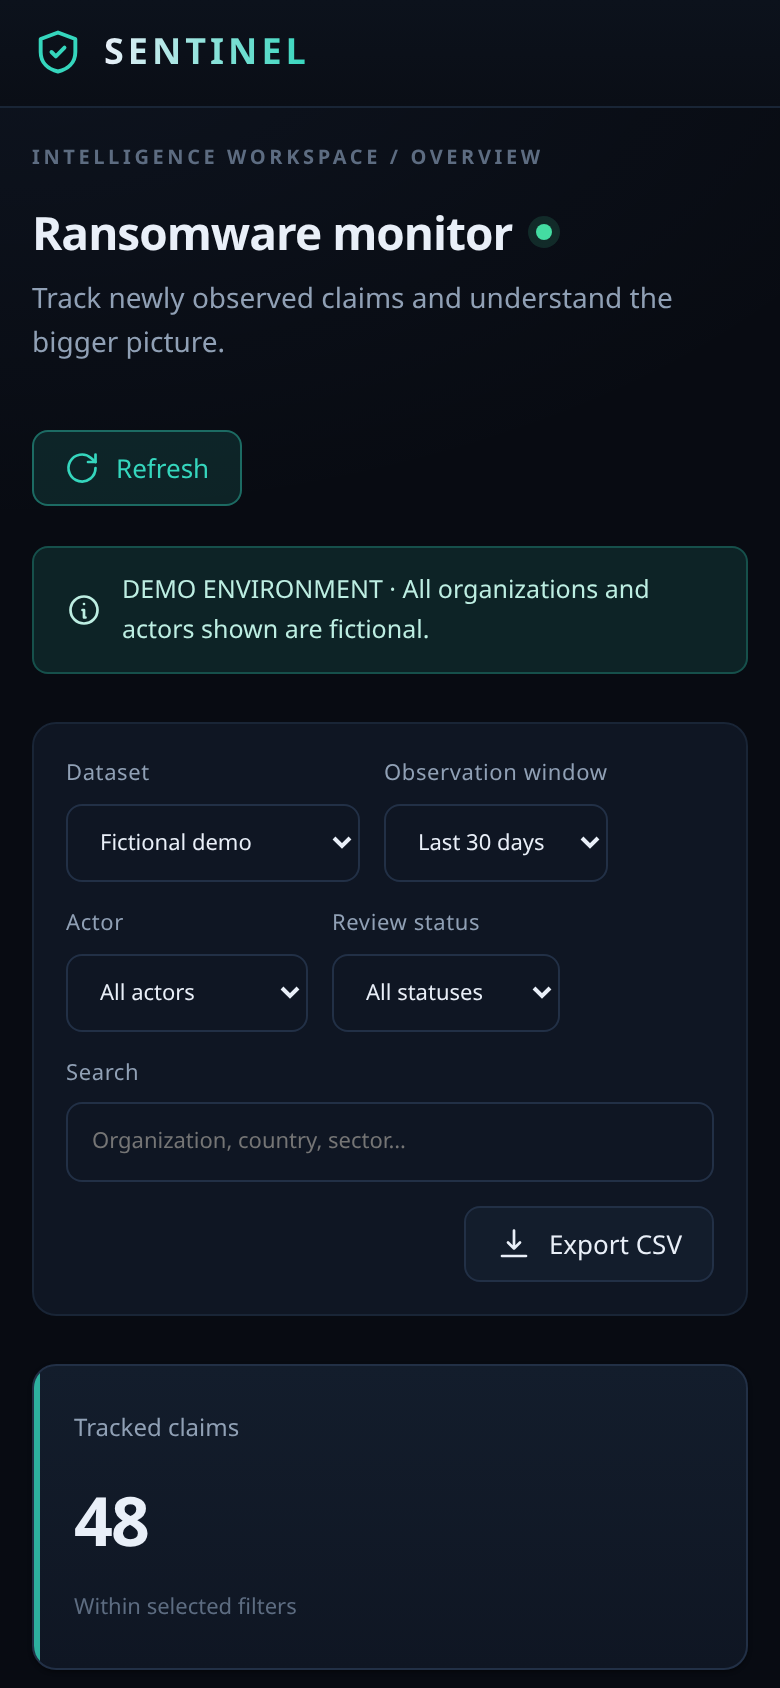
\includegraphics[height=0.55\textheight]{figures/06_mobile.png}
\caption{Phone-width layout (390\,px): the sidebar becomes a header and controls reflow.}
\end{figure}

% ------------------------------------------------------------ 8
\section{Security Analysis}
Sentinel handles untrusted text from adversarial sources, so it is designed on the assumption that every collected string is hostile.

\begin{table}[H]
\centering
\renewcommand{\arraystretch}{1.2}
\begin{tabularx}{\linewidth}{@{}>{\raggedright\arraybackslash}p{3.6cm} X@{}}
\toprule
\textbf{Threat} & \textbf{Mitigation} \\
\midrule
Malicious markup in listings & All source text rendered through DOM text nodes; strict CSP (\code{default-src 'self'}, no inline script or style, \code{frame-ancestors 'none'}) \\
SQL injection & Bound parameters on every query \\
Spreadsheet formula injection & CSV export prefixes cells beginning with \code{=}, \code{+}, \code{-}, \code{@} \\
Cross-site request forgery & POST requires JSON content type and a matching \code{Origin}; Host header must be local \\
Remote exposure & Loopback bind only; documented as not internet-facing \\
SSRF and open redirects & Provider endpoint allowlist, no redirect following, credentials in URLs rejected \\
DNS leakage over Tor & \code{socks5h} enforced; onion URLs rejected without it \\
Resource exhaustion & Response size, time, and record-count caps; sequential requests with delays \\
Secret disclosure & API key read from environment; errors sanitized; exit IP not retained \\
Leaked content handling & Never fetched; only metadata fields stored \\
Lost updates & Version-checked writes and append-only audit history \\
\bottomrule
\end{tabularx}
\caption{Threats and controls.}
\end{table}

\subsection{Operational boundaries}
The application has no authentication, roles, notifications, retention job, or tamper-proof evidence archive, and assessment history is not attributed to authenticated users. It must not be exposed publicly. Source configuration is trusted operator input. A team deployment would require a production web server, authenticated API, TLS, and destination restrictions on collection targets.

% ------------------------------------------------------------ 9
\section{Testing and Quality Assurance}
The suite contains 48 \code{unittest} cases across five modules and passes in about three seconds. Line and branch coverage measured with \code{coverage} is 91\%.

\begin{table}[H]
\centering
\renewcommand{\arraystretch}{1.15}
\begin{tabular}{@{}l r@{}}
\toprule
\textbf{Module} & \textbf{Coverage} \\
\midrule
\code{store.py} & 95\% \\
\code{tor.py} & 96\% \\
\code{providers.py} & 94\% \\
\code{collector.py} & 92\% \\
\code{monitor.py} & 92\% \\
\code{server.py} & 86\% \\
\code{\_\_main\_\_.py} & 84\% \\
\midrule
\textbf{Total} & \textbf{91\%} \\
\bottomrule
\end{tabular}
\caption{Measured coverage by module.}
\end{table}

Tests cover case-insensitive duplicate detection, preservation of first observation, demo/live isolation, atomic rejection of invalid batches, HTML and provider parsing, malformed feeds, onion proxy policy and checksum validation, HTTP routes, cross-origin write rejection, optimistic-concurrency conflicts, schema migration, and CSV neutralization. Tests use temporary databases and a loopback server; they never contact live leak sites. The coverage figure measures executed code, not real-world detection accuracy.

\subsection{Continuous integration}
A GitHub Actions workflow runs the suite on Python 3.11 through 3.14, prints coverage, syntax-checks the JavaScript with Node, builds the package, and verifies that the wheel contains the dashboard assets. The workflow is configured; this report does not claim a hosted run has already succeeded.

% ------------------------------------------------------------ 10
\section{Deployment and Usage}
\begin{lstlisting}[language=bash]
python3 -m venv .venv && source .venv/bin/activate
python -m pip install -e .
python -m sentinel demo          # fictional data
python -m sentinel serve         # http://127.0.0.1:8000

# live public feed + dashboard
python -m sentinel monitor

# direct onion monitoring through a local Tor client
docker compose -p sentinel-tor -f deployment/tor/compose.yml up --build -d
python -m sentinel tor-check
python -m sentinel monitor --config config/sources.darkweb.json
\end{lstlisting}

% ------------------------------------------------------------ 11
\section{Limitations}\label{sec:limits}
\begin{itemize}
  \item Claims are unverified; the same organization under variant names may appear as separate claims.
  \item A recent-items feed can miss records during outages, and trends depend on source coverage and polling timing.
  \item The initial import of an old listing appears as a new observation.
  \item All matching rows are sent to the browser before pagination; aggregates should move into SQL for large datasets.
  \item The authenticated Ransomware.live PRO connector and generic HTML adapters are unverified against live services.
  \item Single-user and local only: no authentication, retention policy, or immutable evidence store.
\end{itemize}

\section{Future Work}
\begin{itemize}
  \item Move filtering, pagination, and aggregation into SQL with indexed queries.
  \item Fuzzy matching and alias tables to merge name variants and repeat incidents.
  \item Authenticated multi-user mode with attributed, tamper-evident audit history.
  \item Outbound notifications for watchlist matches.
  \item A migration framework and a retention policy.
  \item Fixture-based verification of each additional source layout before enabling it.
\end{itemize}

\section{Conclusion}
Sentinel demonstrates a careful approach to a sensitive domain: it observes public claims, keeps strict boundaries around what is collected and how, labels uncertainty plainly, and gives analysts a disciplined workflow for review. The standard-library-first design keeps the codebase small and auditable, and the security controls are tested rather than assumed.

\appendix
\section{Repository Layout}
\begin{lstlisting}
config/        source presets (example, live, darkweb)
data/          SQLite database (git-ignored)
deployment/    Dockerized Tor client
docs/          architecture, validation, guides, this report
scripts/       wheel verification
sentinel/      application package and static dashboard
tests/         unittest suites
\end{lstlisting}

\section{References}
\begin{itemize}
  \item Requests documentation: proxies and SOCKS remote DNS. \url{https://requests.readthedocs.io/en/stable/user/advanced/}
  \item Python \code{sqlite3}: parameter substitution and transactions. \url{https://docs.python.org/3.11/library/sqlite3.html}
  \item Tor Project rendezvous specification, v3 onion addresses. \url{https://spec.torproject.org/rend-spec/}
\end{itemize}

\end{document}
